\documentclass[12pt,a4paper]{scrartcl}
\usepackage[utf8]{inputenc}
\usepackage[ngerman]{babel}
\usepackage{amsmath}
\usepackage{amsfonts}
\usepackage{amssymb}
\usepackage{graphicx}
\usepackage{siunitx}
\usepackage{esvect}
\usepackage{multirow}%Tabellenzellen verbinden
\usepackage{tabulary}%tolle Tabellen
\usepackage{enumitem}%Aufzählungen schöner
\usepackage{dsfont}%Zahlenmengensymbole
\usepackage{pdfpages}
\usepackage[left=1.5cm,right=1.5cm,top=2cm,bottom=3cm]{geometry}
\usepackage{hyperref}
\author{\large
\begin{tabular}{llr}
Malte Hamann & 6318952 &1hamann@informatik.uni-hamburg.de
\\ Evelyn Fischer & 0000000 & 3fischer@informatik.uni-hamburg.de
\\ Marco Jendryczko & 6330073 & 5jendryc@informatik.uni-hamburg.de
\\ Kai Frederking & 6322593 & 1frederk@informatik.uni-hamburg.de
\end{tabular}
}
\title{Übungen Vertiefung Kombinatorische Optimierung Sommersemester 2016\\\vspace{\baselineskip}\large Gruppe 2, Mo 10-12, Abgabe Blatt 01 \\Übungsleiter: \url{daniel.weissauer@uni-hamburg.de}}
\date{\today}

\newcommand{\prob}[1]{\vspace{.5\baselineskip}\begin{addmargin}[15pt]{0pt}\textbf{#1}\end{addmargin}}
\newcommand{\ein}[1]{\vspace{.5\baselineskip}\begin{addmargin}[15pt]{0pt}\textbf{Eingabe: }#1\end{addmargin}}
\newcommand{\fra}[1]{\vspace{.5\baselineskip}\begin{addmargin}[15pt]{0pt}\textbf{Frage: }#1\end{addmargin}}
\newcommand{\loesung}[1]{\vspace{.5\baselineskip}\begin{addmargin}[0pt]{0pt}\textbf{Lösung: }#1\end{addmargin}}

\newcommand{\pr}{$\leq_p$ }%polynomiell reduzierbar


\begin{document}
\maketitle
\vspace{-\baselineskip}
\hrule
\vspace{\baselineskip}
\textbf{Hausaufgaben zum 18. April 2016}
\begin{enumerate}
	\item
	\begin{enumerate}
	\item Als bekannt setzen wir voraus, dass 3D-Matching ein NP-vollständiges Problem ist. Entsprechend zu 3D-MATCHING definiert man $k$D-MATCHING für $k \geq 2$. Formulieren Sie das Problem 4D-MATCHING und zeigen Sie, dass 4D-MATCHING ein NP-vollständiges Problem ist.
	
	\loesung{4D-Matching:
	\ein{Disjunkte Mengen $A$, $B$, $C$ und $D$ mit $|A| = |B| = |C| = |D| = n$ sowie eine Menge $T \subseteq A \times B \times C \times D$ von Tupeln}
	
	\fra{Gibt es eine Menge von $n$ Tupeln in T, so dass jedes Element aus $A \cup B \cup C \cup D$ in genau einem dieser Tupel vorkommt.}
	Zu zeigen:\\
	1. 4D-Matching liegt in NP:\\
	Als Zertifikat gegeben sei ein 4-D Matching $T' \subseteq A \times B \times C \times D$.
	Zu prüfen ist:\\
	$T' \subseteq T$ (möglich in polynomieller Zeit) \\
	$T'$ enthält alle Elemente von $A \cup B \cup C \cup D$ genau ein Mal:\\
	Hierzu prüfen wir, ob $|T'| = n$ ($T'$ muss genau n Tupel enthalten, um die Bedingung erfüllen zu können)\\
	Dann sortieren wir alle Elemente der Tupel in ihrer jeweiligen Dimension aufsteigend ($O(n \cdot \log n)$), durchlaufen alle Dimensionen (4n Aufwand) und prüfen auf doppelt vorkommende Elemente. Finden wir keine, so hält das Zertifikat.\\
	
		
	2. 4d-Matching ist NP-schwer:\\
	Um dies zu zeigen, reduzieren wir 3D-Matching auf 4D-Matching:\\
	Gegeben sei eine Instanz I von 3D-Matching, $I \subseteq A \times B \times C$. Wir konstruieren die dazu gehörige Instanz I' von 4D-Matching, indem wir alle C-Elemene der Tripel als D-Elemente der Quadrupel kopieren.\\
	Behauptung: Die konstruierte Instanz I' besitzt ein 4D-Matching, g.d.w. I ein 3D-Matching besitzt.\\
	``$\Rightarrow$'': Da für ein 4-D Matching alle A-, B- und C-Elemente genau einmal enthalten sein müssen (ebenso wie die D-Elemente), folgt das 3D-Matching von I aus dem 4D-Matching von I'.\\
	``$\Leftarrow$'': Folgt aus der Konstruktion. Wenn alle C-Elemente genau einmal enthalten sind (notwendige Bedingung des 3D-Matching von I), so sind es wegen der Duplizierung auch die D-Elemente von I'.\\ \\
	
					}
	\item Für jedes feste $k \geq 2$ definieren wir das Problem $k$-CLIQUE wie folgt:
	\prob{k-CLIQUE}
	\ein{Ein Graph $G = (V,E)$.}
	\fra{Enthält $G$ einen vollständigen Graphen mit $k$ Knoten?}
	Für welche $k\geq 2$ ist $k$-CLIQUE ein NP-vollständiges Problem?
	
	\textbf{Hinweis:} Zur Lösung von Aufgabe 1 reicht es natürlich nicht, Antworten ohne Begründung zu geben; es kommt darauf an, Antworten zu geben \emph{und deren Richtigkeit nachzuweisen.}
	
	\loesung{Für kein festes k. Solange k fest ist, ist das Problem in P (wenn auch mit teils großen Exponenten). Lediglich für beliebige, nicht-feste k ist das Clique-Problem in NP (und dann NP-vollständig, wie von Karp gezeigt).\\ \\
	Beweis durch Induktion über die Cliquengröße k:
	Für $k = 1$ ist die 1-Clique = V und der Aufwand der Ermittlung $O(n)$, $n = |V|$\\
	Gegeben seien alle k-Cliquen eines Graphen G als lineare Listen der zur jeweiligen Clique gehörigen Knoten. Die Menge der Cliquen sei disjunkt (keine Clique kommt mehr als einmal vor), die Knotenmenge zweier Cliquen kann allerdings nichtleere Schnitte haben (ein Knoten gehört zu verschiedenen Cliquen).\\
	Es kann höchstens $n \choose k$ solcher Cliquen geben, mit ${n \choose k} \leq n^k$.\\
	Zur Ermittlung aller k+1-Cliquen durchlaufen wir jetzt alle k-Cliquen C (höchstens $n^k$), betrachten alle Knoten $v \in V \setminus C$, also die aus V, die noch nicht in C enthalten sind (höchstens n), durchlaufen deren Adjazenzlisten (höchstens n lang) und prüfen, ob alle ihre Elemente in C liegen (höchstens n Vergleiche). Ist dies der Fall, so ist $C \cup \{v\}$ eine k+1-Clique. Andernfalls nicht. Der Aufwand insgesamt ist höchstens $n^k \cdot n \cdot n \cdot n = n^{k+3}$. Hierzu kommt noch die Prüfung, ob eine neu gefundene k+1-Clique bereits auf anderem Wege gefunden wurde, das ändert aber $O(n^{k+3})$ nicht.\\
	Um auf diese Weise alle k-Cliquen eines Graphen iterativ von den 1-Cliquen an zu ermitteln, benötigen wir höchstens\\
	$n \cdot \sum_{i=2}^k n^{i-1+3} = n \cdot \sum_{i=2}^k n^{i+2} \leq n \cdot n^{k+3} = n^{k+4}$\\
	und somit polynomielle Zeit.\\ \\
	}
	%Ich vermute mal, dass es ab k=3 NP-vollständig ist, weil man dann nicht mehr einfach nur eine Kante zwischen zwei beliebigen Knoten brauch, sondern quasi eine SCC mit 3-Knoten.
	%Antwort Kai: Nicht ganz ... siehe oben.				}
	\end{enumerate}

\item Gegeben sei eine Menge $A = \{a_1,\ldots,a_n\}$ sowie eine Kollektion $B_1,\ldots,B_m$ von Teilmengen von $A$. Eine Menge $H \subseteq A$ wird \emph{Hitting Set} für $B_1,\ldots,B_m$ genannt, falls $H \cap B_i \neq \emptyset$ für alle $i \in \{1,\ldots,m\}$ gilt. Wir betrachten das folgende Entscheidungsproblem:

	\prob{HITTING SET}
	\ein{Eine Menge $A = \{a_1,\ldots,a_n\},$ Teilmengen $B_1,\ldots,B_m$ von $A$ sowie eine Schranke $k \in \mathds{Z}, k \geq 1$.}
	\fra{Gibt es ein Hitting Set $H \subseteq A$ für $B_1,\ldots,B_m$, für das $|H| \leq k$ gilt?}
	\begin{enumerate}
	\item Beweisen Sie, dass HITTING SET ein NP-vollständiges Problem ist, indem Sie erstens nachweisen, dass HITTING SET in NP liegt, und zweitens 3-SAT zur Reduktion heranziehen.
	
	\loesung{
	HITTING SET liegt in NP, da bei Vorlegen des Zertifikats H in polynomieller Zeit geprüft werden kann, ob H aus jeder Menge $B_1$ ... $B_m$ mindestens ein Element enthält und selber höchstens k Elemente enthält.\\  \\
	Die Reduktion von 3-SAT auf HITTING SET gelingt folgendermaßen:\\
	Zu einer gegebenen Instanz $\Phi$ von 3-SAT konstruieren wir ein HITTING SET Problem $\Phi'$, so dass A die Menge der Literale enthält, sowie deren Negationen. Die Teilmengen B repräsentieren die Klauseln und enthalten je drei Literale, bzw. negierte Literale. Zusätzlich nehmen wir in B noch für jeden Literal eine 2-elementige Teilmenge auf, die diesen Literal und seine Negation enthält. So stellen wir sicher, dass H jeden Literal oder seine Negation enthalten muss. Wenn wir die Größe von H jetzt noch auf $|A| / 2$ beschränken (indem wir $k = |A| / 2$ wählen), so enthält H bei ``erfolgreichem HIT'' jeden Literal entweder negiert oder nicht negiert.\\ \\
	Behauptung: Die konstruierte Instanz $\Phi'$ besitzt einen k-HITTING SET ($k = |A| / 2$), g.d.w. $\Phi$ eine erfüllende Eingabe besitzt.\\
	``$\Rightarrow$'': Der HITTING SET H enthält keine widersprüchlichen Literale (s.o.). Er enthält mindestens ein Element (negiert oder nicht) aus jeder Klausel, so dass wenn alle Elemente aus H auf wahr gesetzt werden, alle Klauseln erfüllt sind.\\
	``$\Leftarrow$'': Existiert eine erfüllende Belegung, so gehört aus den zweielementigen Teilmengen jeweils die erfüllende Belegung des Literals zu H und jede Klausel enthält von diesen Belegungen mindestens eine, so dass H auch Elemente aus allen Klauseln enthält.\\
	
	}
	
	\item Um die NP-Vollständigkeit von HITTING SET nachzuweisen, muss man nicht unbedingt 3-SAT verwenden. Fällt Ihnen eine andere (möglichst einfache) Reduktion eines NP-vollständigen Problems auf HITTING SET ein?
	
	\loesung{VERTEX COVER erscheint besonders einfach zu sein. Wir nehmen die durch Kanten verbundenen Knoten als (2-elementige) Teilmengen $B_i$. Wenn wir jetzt einen HITTING SET von Größe $\leq$ k finden, dann haben wir auch ein k-VERTEX COVER mit den in H enthaltenen Knoten (da jede Teilmenge eine Kante repräsentiert und wir zu jeder Kante einen inzidenten Knoten in H haben).}
	\end{enumerate}

\end{enumerate}

Illustrationen: \\


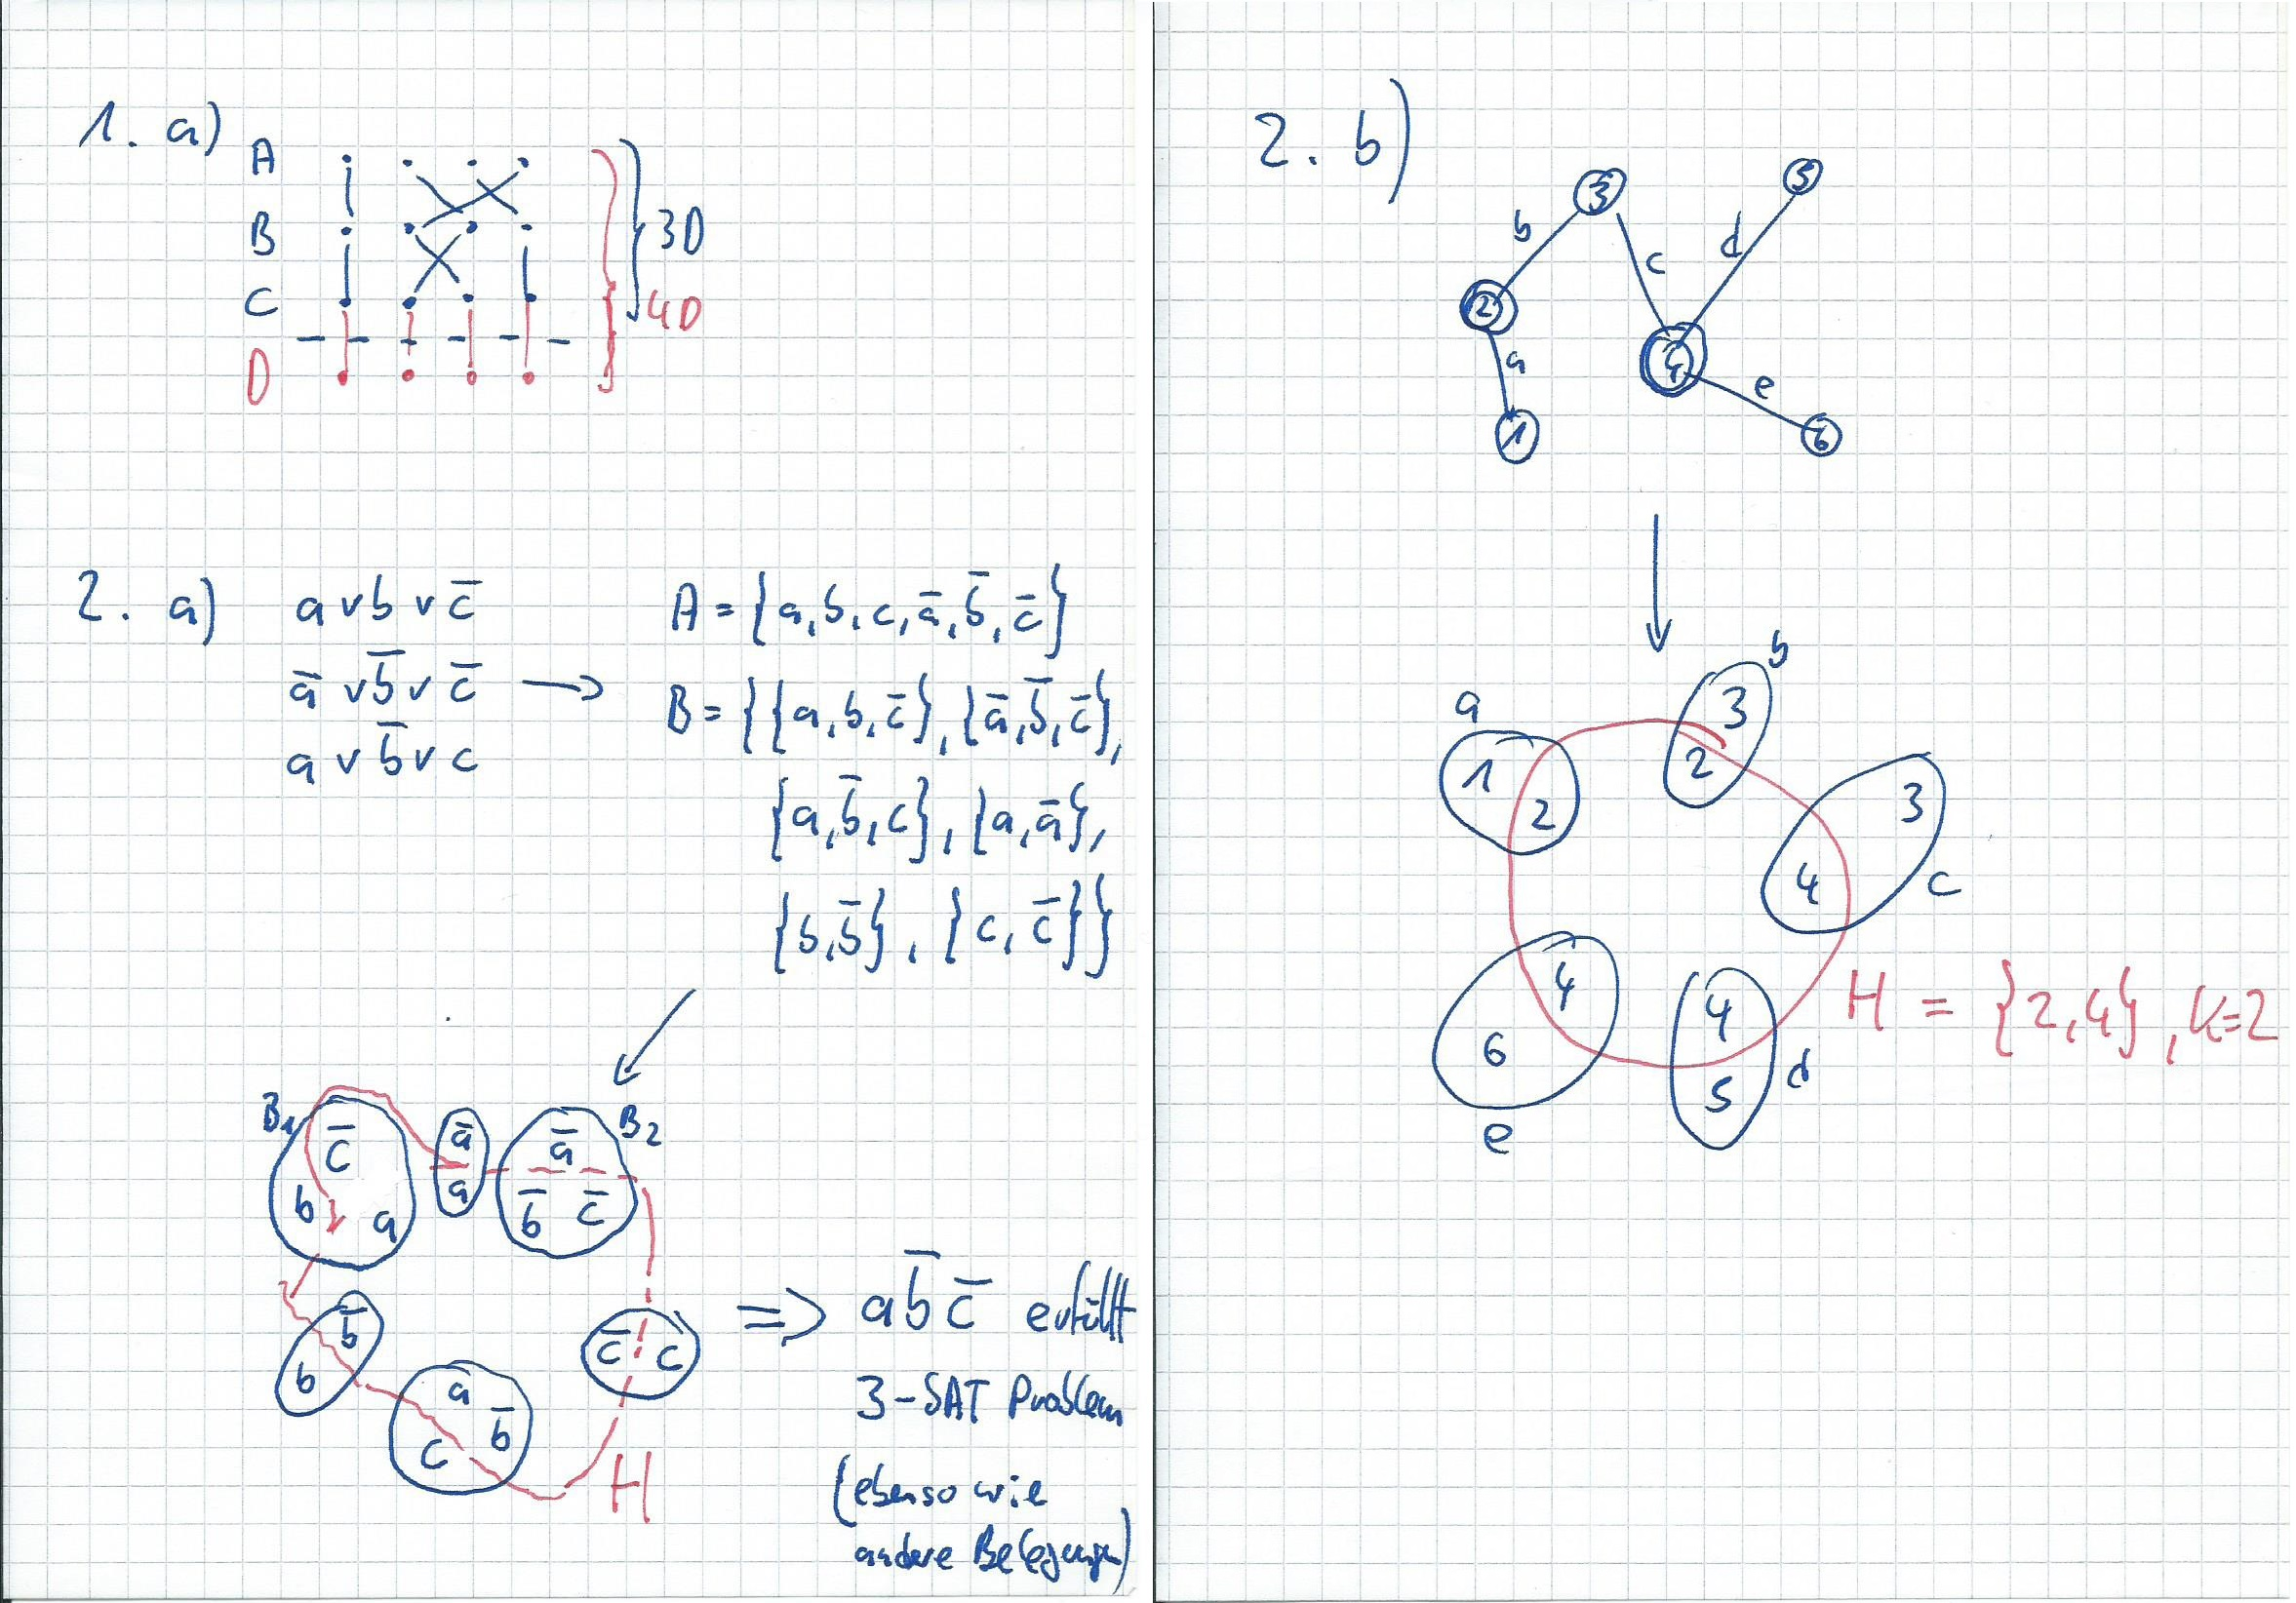
\includegraphics [scale=0.6] {Ueb01_1.jpg}

\end{document}
